\documentclass[a4paper,ngerman,14pt]{scrartcl}

\usepackage[utf8]{inputenc}
\usepackage{amssymb}

\usepackage[ngerman]{babel}
\usepackage{pdfpages}

\usepackage{graphicx}

\usepackage[protrusion=true,expansion=true]{microtype}

\usepackage{hyperref}
\usepackage{lmodern}
\usepackage{tabto}

\setlength\parskip{\medskipamount}
\setlength\parindent{0pt}

\usepackage{geometry}
\geometry{tmargin=1.5cm,bmargin=2cm,lmargin=3cm,rmargin=3cm}

\pagestyle{empty}

\setlength{\fboxrule}{2pt}
\setlength{\fboxsep}{-3pt}

\newcommand{\drawHere}{%
  \begin{center}%
    \fbox{\parbox[c][0.9\textwidth]{0.9\textwidth}{\ }}%
  \end{center}}

\newcommand{\header}[1]{\begin{center}
  \Huge\textbf{\textsf{#1}}
\end{center}}

\renewcommand{\labelitemi}{$\bigstar$}

\begin{document}

\header{Das Binärsystem}

Im gewöhnlichen Zehnersystem gibt es die Ziffern von~$0$ bis~$9$. Der Wert 
einer Ziffer ergibt sich von rechts nach links über die Zehnerpotenzen: Einer,
Zehner, Hunderter, Tausender, usw.

Das Binärsystem ist viel einfacher: Da gibt
es nur die Ziffern~$0$ und~$1$. Der Wert einer Ziffer ergibt sich dann von
rechts nach links über die Zweierpotenzen: Einer, Zweier, Vierer, Achter,
Sechzehner, usw.

\begin{enumerate}
\item Erkläre folgende Beispiele!

\begin{center}
\begin{tabular}{r|l}
  Binärdarstellung & Dezimaldarstellung \\\hline
  1 & 1 \\
  10 & 2 \\
  11 & 3 \\
  100 & 4 \\
  101 & 5 \\
  1010 & 10
\end{tabular}
\end{center}

\item Welche Zahl bezeichnet die Binärdarstellung~$111$?
\item Wie schreibt sich deine Lieblingszahl im Binärsystem?
\item Wie kann man im Binärsystem ganz einfach eine Zahl verdoppeln?
\item Addiere zwei Zahlen deiner Wahl im Binärsystem! Das geht ganz ähnlich wie
bei der üblichen schriftlichen Addition.
\end{enumerate}

\newpage

\header{Nim}

Mehrere Haufen von Spielsteinen liegen auf dem Tisch. Zwei Spieler dürfen
sich abwechselnd einen Haufen aussuchen und müssen dann von diesem beliebig viele,
mindestens jedoch einen Stein entfernen. Verlierer ist, wer keinen Zug mehr
tätigen kann; es gewinnt also der, der den letzten Stein wegnehmen kann.

\begin{enumerate}
\item Spiele Nim einige Male, um ein Gefühl für das Spiel zu entwickeln!
\item Wenn es nur noch einen Haufen gibt, kann immer der Spieler gewinnen, der
anfängt. Wieso?
\item Wenn es nur noch zwei Haufen gleicher Größe gibt, kann immer einer der
beiden Spieler gewinnen. Welcher?
\item Wenn es nur noch zwei Haufen gibt, wobei der eine Haufen größer als der
andere ist, kann ebenfalls ein bestimmter Spieler immer gewinnen. Wer?
\item Addiere bei all diesen Beispielen die Größen der
Haufen -- aber nicht wie üblich, sondern \emph{im Binärsystem} und \emph{ohne
Übertrag}. Was fällt auf? Rechne noch mehr Beispiele!
\item Erkläre, wie man daher mithilfe des Binärsystems optimal spielen kann!
\end{enumerate}

\newpage

\header{Das Hunderterspiel}

Zwei Spieler beginnen mit der Gesamtsumme Null. Dann
dürfen die Spieler abwechselnd eine Zahl zwischen Eins und Zehn auf die Summe
addieren. Wer die Summe auf Hundert bringen kann, gewinnt.

\begin{enumerate}
\item Spiele das Hunderterspiel einige Male, um ein Gefühl für das Spiel zu
entwickeln!
\item Angenommen, du bist an der Reihe und sagst die Zahl~$89$. Wieso
hast du dann garantiert gewonnen?
\item Findest du weitere Zahlen dieser Art, die dir mit Sicherheit zum Gewinn
verhelfen?
\item Was hat das Hunderterspiel mit dem Münzspiel zu tun?
\end{enumerate}

\newpage

\header{Rim}

Rim spielt man mit Pünktchen auf Papier. Das Spielfeld kann zum Beispiel so
aussehen:
\begin{center}
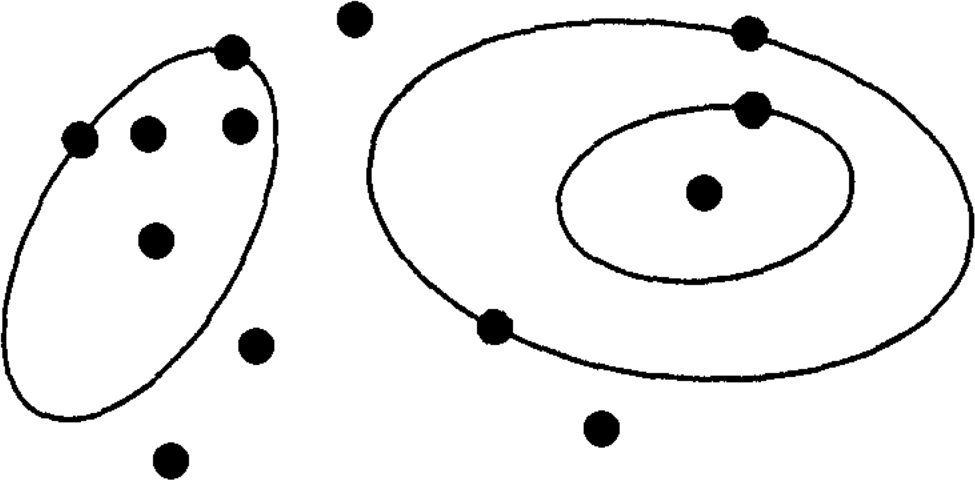
\includegraphics[scale=0.3]{../rim}
\end{center}
Wie Nim spielen bei Rim zwei Spieler gegeneinander.
Wenn ein Spieler am Zug ist, muss er oder sie
eine geschlossene Linie zeichnen, auf der mindestens ein Pünktchen liegt und
die keine bereits vorhandene Linie kreuzt oder berührt. Verloren hat, wer
keinen Zug mehr tätigen kann.

\begin{enumerate}
\item Spiele Rim einige Male, um ein Gefühl für das Spiel zu entwickeln!
\item Finde heraus, was Rim mit Nim zu tun hat!
\item Wenn du die optimale Strategie für Nim kennst, dann weißt du daher auch,
wie man Rim optimal spielt. Erkläre, wie das geht!
\end{enumerate}


\end{document}

\begin{enumerate}
\item Wenn du am Zug bist, addiere die Werte der Haufen im Binärsystem
\emph{ohne Übertrag}.
\item Wenn diese Summe Null ist, kann leider dein Gegenspieler einen Sieg
erzwingen. In diesem Fall besteht die einzige Gewinnmöglichkeit darin, einen möglichst
unübersichtlichen Zug zu tätigen, um deinen Gegner zu verwirren.
\item Wenn diese Summe nicht Null ist, überlege, welchen Haufen man
verändern muss, damit die neue Summe doch Null wird. Führe dann genau diesen
Zug aus.
\end{enumerate}
